\section{Модификации DQN}\label{sec:dqnmods}

\subsection{Twin DQN}

Отмечалось, что без таргет-сетки (при обновлении задачи регрессии каждый шаг) можно наблюдать, как $Q^*$ начинает неограниченно расти. Хотя таргет-сетка более-менее справляется с тем, чтобы стабилизровать процесс, предотвратить этот эффект полностью у неё не получается: сравнение обучающейся $Q^*$ с Монте-Карло оценками и зачастую просто со здравым смыслом выдаёт присутствие в алгоритме заметного \emph{смещения в сторону переоценки} (overestimation bias). Почему так происходит?

Очевидно, что источник проблемы --- оператор максимума в формуле построения таргета: 
$$y(\T ) = r + \gamma \max\limits_{a'} Q^*(s', a', \theta^-)$$
При построении таргета есть два источника ошибок: 1) ошибка аппроксимации 2) внешняя стохастика. Максимум здесь <<выбирает>> то действие, для которого из-за ошибки нейросети или из-за везения в прошлых играх $Q(s', a')$ больше правильного значения.

\begin{example}
Вы выиграли в лотерею +100. Из-за того, что вы моделируете Q-сетку нейросетью, при увеличении $Q(s, a)$ для действия <<купить билет в лотерею>> случайно увеличилось значение $Q(s, a)$ для действия <<играть с \href{https://ru.wikipedia.org/wiki/Слот-машина}{однорукими бандитами}>>, поскольку оно опиралось на примерно те же признаки описания состояний. В результате, при построении таргета для состояния казино $s'$ в задачу регрессии поступают завышенные значения, которые дальше распространяются на другие состояния: начинается <<цепная реакция>>.
\end{example}

Одно из хороших решений проблемы заключается в разделении (decoupling) двух этапов подсчёта максимума: \emph{выбор действия} (action selection) и \emph{оценка действия} (action evaluation):
$$\max\limits_{a'} Q^*(s', a') = \overbrace{Q^*(s', \underbrace{\argmax\limits_{a'} Q^*(s', a')}_{\text{выбор действия}})}^{\text{оценка действия}}$$

В Twin DQN\footnote{когда эту идею предлагали в 2010-ом году в рамках классического RL (тогда нейронки ещё не вставили), то назвали её Double Q-learning, но сейчас под Double DQN подразумевается алгоритм 2015-го года, а этот трюк иногда именуется <<близнецами>> (Twin). Правда, в последнее время из-за алгоритма Twin Delayed DDPG под словом Twin понимается снова не эта формула...} предлагается обучать два приближения Q-функции параллельно и использовать аппроксимацию Q-функции <<близнеца>> для этапа оценивания действия:
$$\textcolor{ChadBlue}{y_1}(\T ) \coloneqq r + \gamma \textcolor{ChadBlue}{Q_{\theta_1}^*}(s', \argmax\limits_{a'} \textcolor{ChadPurple}{Q_{\theta_2}^*}(s', a'))$$
$$\textcolor{ChadPurple}{y_2}(\T ) \coloneqq r + \gamma \textcolor{ChadPurple}{Q_{\theta_2}^*}(s', \argmax\limits_{a'} \textcolor{ChadBlue}{Q_{\theta_1}^*}(s', a'))$$

Если обе аппроксимации Q-функции идеальны, то, понятное дело, мы всё равно получим честный максимум. Однако, если оба DQN честно запущены параллельно и даже собирают каждый свой опыт (что в реальности, конечно, дороговато), их ошибки аппроксимации и везения будут в <<разных местах>>. В итоге, Q-функция близнеца выступает в роли более пессимистичного критика действия, выбираемого текущей Q-функцией. Таргет-сети в такой модели не нужны, то есть задача регрессии, условно говоря, меняется после каждого обновления весов.

\begin{remark}
Если сбор уникального опыта для каждого из близнецов не организуется, Q-функции всё равно получаются скоррелированными. Как минимум, нужно сэмплировать для обучения сеток разные мини-батчи из реплей буфера, если он общий.
\end{remark}

Интуиция, почему <<независимая>> Q-функция близнеца используется именно для оценки действия, а не наоборот для выбора: если из-за неудачного градиентного шага наша сетка $Q_{\theta_1}$ пошла куда-то не туда, мы не хотим, чтобы плохие значения попадали в её же таргет. Плохие действия в таргет пусть попадают: пессимистичная оценка здесь предпочтительнее.

\subsection{Clipped Twin DQN}

Разовьём интуицию дальше. Вот мы строим таргет для $Q_{\theta_1}$. Мы готовы выбрать при помощи неё же действия, но не готовы оценить их ею же самой в силу потенциальной переоценки. Для этого мы и берём <<независимого близнеца>> $Q_{\theta_2}$. Но что, если он выдаёт ещё больше? Что, если его оценка выбранного действия, так случилась, потенциально ещё более завышенная? Давайте уж в таких ситуациях всё-таки брать то значение, которое поменьше! Получаем следующую интересную формулу:
$$\textcolor{ChadBlue}{y_1}(\T ) \coloneqq r + \gamma \min_{i = \textcolor{ChadBlue}{1}, \textcolor{ChadPurple}{2}}Q_{\theta_i}^*(s', \argmax\limits_{a'} \textcolor{ChadPurple}{Q_{\theta_2}^*}(s', a'))$$
$$\textcolor{ChadPurple}{y_2}(\T ) \coloneqq r + \gamma \min_{i = \textcolor{ChadBlue}{1}, \textcolor{ChadPurple}{2}}Q_{\theta_i}^*(s', \argmax\limits_{a'} \textcolor{ChadBlue}{Q_{\theta_1}^*}(s', a'))$$

Мы по сути придумали забавный метод <<ансамблирования>> Q-функций: только вместо интуитивного среднего берём минимум, для борьбы с максимумом. 

\begin{remark}
Конечно, в отличие от обычного ансамблирования в машинном обучении, такой подход плохо масштабируется с увеличением числа обучаемых Q-функций (обычно учат всё-таки только две). В случае ансамбля имеет смысл брать не среднее, и не минимум, а, например, какой-то квантиль, более близкий к минимуму, чем к медиане --- но возникает неудобный гиперпараметр, что же именно брать.
\end{remark}

\subsection{Double DQN}\label{subsec:doubledqn}

Запускать параллельно обучение двух сеток дороговато, а при общем реплей буфере корреляция между ними всё равно будет. Поэтому предлагается простая идея: запускать лишь один DQN, а в формуле таргета для оценивания вместо <<близнеца>> использовать таргет-сеть. То есть: пусть $\theta$ --- текущие веса, $\theta^{-}$ --- веса таргет-сети, раз в $K$ шагов копирующиеся из $\theta$. Тогда таргет вычисляется по формуле:
$$y(\T ) \coloneqq r + \gamma Q^*(s', \argmax\limits_{a'} Q^*(s', a', \theta), \theta^-)$$

Хотя понятно, что таргет-сеть и текущая сетка очень похожи, такое изменение формулы целевой переменной всё равно <<избавляет>> нас от взятия оператора максимума; эмпирически оказывается, что такая декорреляция действительно помогает стабилизации процесса. При этом, в отличие от предыдущих вариантов, такое изменение бесплатно: не требует обучения второй нейросети.

\subsection{Dueling DQN}\label{subsec:duelingdqn}

Рассмотрим ещё одну очевидную беду Q-обучения на примере. 

\begin{example}
Вы в целях исследования попробовали кинуться в яму $s$. Сидя в яме, вы попробовали $a$ --- поднять правую руку. В яме холодно и грустно, поэтому вы получили -100. Какой вывод делает агент? Правильно: для этого состояния $s$ оценку этого действия $a$ нужно понизить. Остальные не трогать; оценка самого состояния (по формуле \eqref{V*Q*} --- максимум Q-функции по действиям) скорее всего не изменится, и надо бы вернуться в это состояние и перепроверить ещё и все остальные действия: попробовать поднять левую руку, свернуться калачиком...
\end{example}

В сложных MDP ситуация зачастую такова, что получение негативной награды в некоторой области пространства состояний означает в целом, что попадание в эту область нежелательно. Верно, что с точки зрения теории остальные действия должны быть <<исследованы>>, но неудачный опыт должен учитываться внутри оценки самого состояния; иначе агент будет возвращаться в плохие состояния с целью перепробовать все действия без понимания, что удача здесь маловероятна, вместо того, чтобы исследовать те ветки, где негативного опыта <<не было>>. Понятно, что проблема тем серьёзнее, чем больше размерность пространства действий $|\A|$.

\needspace{7\baselineskip}
\begin{wrapfigure}{r}{0.4\textwidth}
\vspace{-0.3cm}
\centering
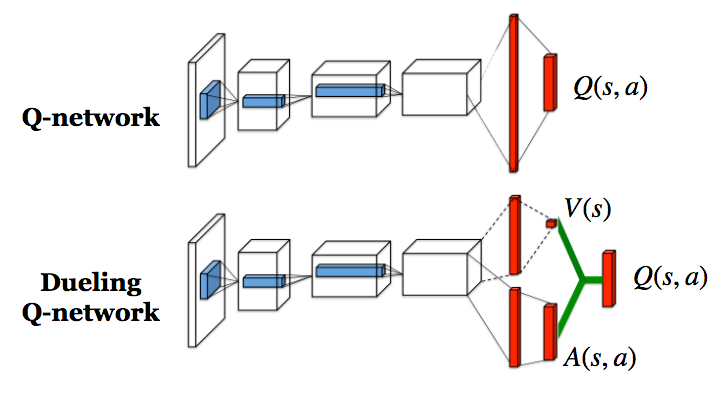
\includegraphics[width=0.4\textwidth]{Images/DuelingDQN.png}
\vspace{-0.3cm}
\end{wrapfigure}

Формализуя идею, мы хотели бы в модели учить не $Q^*(s, a)$ напрямую, а получать их с учётом $V^*(s)$. Иными словами, модель должна знать ценность самих состояний и с её учётом выдавать ценности действий. \emph{Дуэльная} (\ENGLISH{dueling}) архитектура --- это модификация вычислительного графа нашей модели с параметрами $\theta$, в которой на выходе предлагается иметь две головы, V-функцию $V^*$ и Advantage-функцию $A^*$: 
\begin{equation}\label{naivedueling}
Q^*(s, a, \theta) \coloneqq V^*(s, \theta) + A^*(s, a, \theta)
\end{equation}

Здесь есть проблема: если $V^*(s, \theta)$ --- это произвольный скаляр, то $A^*(s, a, \theta)$ --- не произвольный. \ENGLISH{Advantage}-функция не является произвольной функцией и обязана подчиняться \eqref{pr:advantageiszero}. Для оптимальных стратегий в предположении жадности нашей стратегии это утверждение вырождается в следующее свойство:
\begin{proposition}
$$\forall s \colon \max_a A^*(s, a) = 0$$
\beginproof
\begin{align*}
    \max_a A^*(s, a) = \max_a Q^*(s, a) - V^*(s) = \{ \text{V*Q* \eqref{V*Q*}} \} = 0 \tagqed
\end{align*}
\end{proposition}
Это условие можно легко учесть, вычтя максимум в формуле \eqref{naivedueling}:
\begin{equation}\label{dueling}
Q^*(s, a, \theta) = V^*(s, \theta) + A^*(s, a, \theta) - \max_{\hat{a}} A^*(s, \hat{a}, \theta)    
\end{equation}
Таким образом мы гарантируем, что максимум по действиям последних двух слагаемых равен нулю, и они корректно моделируют Advantage-функцию.

Заметим, что $V^*$ и $A^*$ не учатся по отдельности (для $V^*$ уравнение оптимальности Беллмана не сводится к регрессии, для $A^*$ уравнения Беллмана не существует вообще); вместо этого минимизируется лосс для Q-функции точно так же, как и в обычном DQN.

\begin{remark}
В нейросетях формулу \eqref{dueling} реализовать очень просто при помощи двух голов: одна выдаёт скаляр, другая $|\A|$ чисел, из которых вычитается максимум. Дальше к каждой компоненте второй головы добавляется скаляр, выданный первой головой, и результат считается выданным моделью $Q^*(s, a, \theta)$. Преимущество модели остаётся в том, что при апдейте значения для одной пары $s, a$ неизбежно поменяется значение $V^*(s, \theta)$ ценности всего состояния, и ценность <<всех действий>> сразу упадёт.
\end{remark}

Нюанс: авторы статьи эмпирически обнаружили, что замена максимума на среднее даёт чуть лучшие результаты. В результате, на текущий день под дуэльной архитектурой понимают альтернативную формулу:
\begin{equation}\label{kludgedueling}
Q^*(s, a, \theta) = V^*(s, \theta) + A^*(s, a, \theta) - \frac{1}{|\A|}\sum_{\hat{a}} A^*(s, \hat{a}, \theta)    
\end{equation}

\subsection{Шумные сети (Noisy Nets)}\label{subsec:noisynets}

По дефолту, алгоритмы на основе DQN никак не пытаются решать дилемму исследования-использования и просто используют $\eps$-жадную стратегию взаимодействия со средой. Этот бэйзлайн-подход плох примерно всем, в первую очередь тем, что крайне чувствителен к гиперпараметрам: раннее затухание приведёт к застреванию алгоритма в локальном оптимуме (агент будет биться головой об стенкой, не пробуя её обойти), а слишком большие значения существенно замедляют обучение, заставляя агента вести себя случайно. 

\needspace{7\baselineskip}
\begin{wrapfigure}{r}{0.4\textwidth}
\vspace{-0.3cm}
\centering
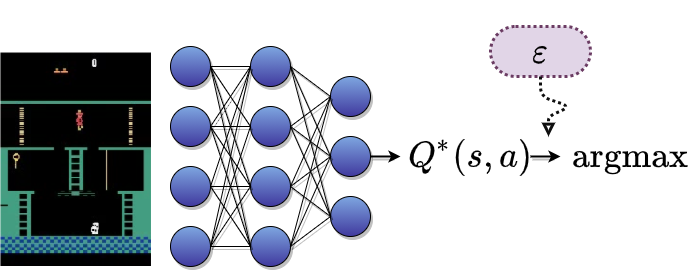
\includegraphics[width=0.4\textwidth]{Images/NoisyNets1.png}
\vspace{-0.3cm}
\end{wrapfigure}

Ключевая причина, почему $\eps$-жадная стратегия примитивна, заключается в независимости добавляемого шума от текущего состояния. Мы выдаём оценки Q-функции и в зависимости только от времени принимаем решение, использовать ли эти знания или эксплорить. Интуитивно, правильнее было бы принимать это решение в зависимости от текущего состояния: если состояние исследовано, чаще принимать решение в пользу использования знаний, если ново --- в пользу исследования. Открытие новой области пространства состояний скорее всего означает, что в ней стоит поделать разные действия, когда двигаться к ней нужно за счёт использования уже накопленных знаний.

\needspace{7\baselineskip}
\begin{wrapfigure}{l}{0.4\textwidth}
\vspace{-0.3cm}
\centering
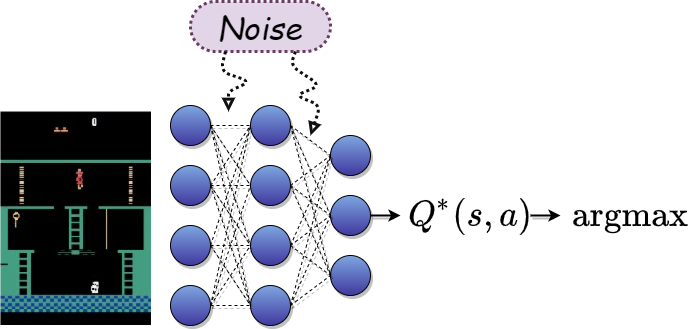
\includegraphics[width=0.4\textwidth]{Images/NoisyNets2.png}
\vspace{-0.3cm}
\end{wrapfigure}

\emph{Шумные сети} (\ENGLISH{noisy nets}) --- добавление шума с обучаемой и, главное, зависимой от состояния (входа в модель) дисперсией. Хак чисто инженерный: давайте каждый параметр в модели заменим на
$$\theta_i \coloneqq w_i + \sigma_i \eps_i \qquad \eps_i \sim \N(0, 1),$$
или, другими словами, заменим веса сети на сэмплы из $\N(w_i, \sigma^2_i)$, где $w, \sigma \in \R^h$ --- параметры модели, обучаемые градиентным спуском. Очевидно, что выход сети становится случайной величиной, и, в зависимости от шума $\eps$, будет меняться выбор действия $a \HM= \argmax\limits_a Q^*(s, a, \theta, \eps)$. При этом влияние шума на принятое решение зависит от состояния.

\begin{remark}
Если состояния --- изображения, шум в свёрточные слои обычно не добавляется (зашумлять выделение объектов из изображения кажется бессмысленным).
\end{remark}

Формально, коли наша модель стала стохастичной, мы поменяли оптимизируемый функционал: мы хотим минимизировать функцию потерь в среднем по шуму:
$$\E_{\eps} \Loss(\theta, \eps) \to \min_\theta$$
Видно, что градиент такого функционала можно несмещённо оценивать по Монте-Карло:
$$\nabla_\theta \E_{\eps} \Loss(\theta, \eps) = \E_{\eps} \nabla_\theta \Loss(\theta, \varepsilon) \approx \nabla_\theta \Loss(\theta, \eps) \quad \eps \sim \N(0, I)$$

Гарантий, что магнитуда шума в среднем будет падать для исследованных состояний, вообще говоря, нет. Надежда этой идеи в том, что магнитуда будет подстраиваться в зависимости от текущих в модель градиентов, при этом гиперпараметры в подходе отсутствуют.
\begin{remark}
Кроме инициализации. Неудачная инициализация $\sigma$ всё равно может замедлить процесс обучения; обычно дисперсию шума инициализируют какой-нибудь константой, и эта константа становится в некотором смысле важным гиперпараметром алгоритма.
\end{remark}

\begin{remark}
Генерация сэмплов шума по числу параметров нейросети на видеокарте может сильно замедлить время прохода через сеть. Для оптимизации авторы предлагают для матриц полносвязных слоёв генерировать шум следующим образом. Пусть $n$ --- число входов, $m$ --- число выходов в слое. Сэмплируются $\eps_1 \sim \N(0, I_{m \times m}), \eps_2 \sim \N(0, I_{n \times n})$, после чего полагается шум для матрицы равным
$$\eps \coloneqq f(\eps_1) f(\eps_2)^T$$
где $f$ --- масштабирующая функция, например $f(x) = \operatorname{sign}(x)\sqrt{|x|}$ (чтобы каждый сэмпл в среднем всё ещё имел дисперсию 1). Процедура требует всего $m + n$ сэмплов вместо $mn$, но жертвует независимостью сэмплов внутри слоя.
\end{remark}

\begin{remark}
Альтернативно, можно зашумлять выходы слоёв (тогда сэмплов понадобится на порядок меньше) или просто добавлять шум на вход. В обоих случаях, <<зашумлённость>> выхода будет обучаемой, а степень влияния шума на выход сети будет зависеть от состояния.
\end{remark}

Заметим, что таргет $y(\T)$, который мы генерируем для каждого перехода $\T$ из батча, формально теперь тоже должен вычисляться как мат.ожидание по шуму:
$$y(\T) \coloneqq \E_\eps \left[ r + \gamma \max_{a'} Q^*(s', a', \theta, \eps) \right]$$
Опять же, мат.ожидание несмещённо оценивается по Монте-Карло, однако с целью декорреляции полезно использовать в качестве $\eps$ другие сэмплы, нежели используемые при вычислении лосса.

\subsection{Приоритизированный реплей (Prioritized DQN)}\label{subsec:prioritizedreplay}

\needspace{7\baselineskip}
\begin{wrapfigure}{r}{0.3\textwidth}
\vspace{-0.3cm}
\centering
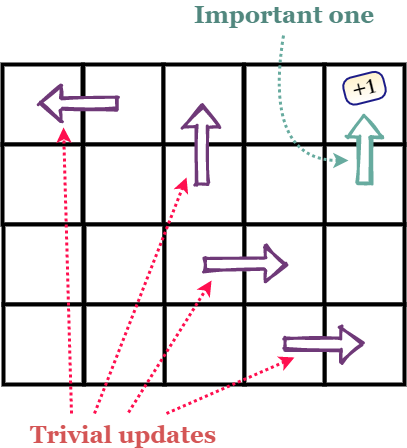
\includegraphics[width=0.3\textwidth]{Images/PER.png}
\vspace{-0.3cm}
\end{wrapfigure}

Off-policy алгоритмы позволяют хранить и переиспользовать весь накопленный опыт. Однако, интуитивно ясно, что встречавшиеся переходы существенно различаются по важности. Зачастую большая часть буфера, особенно поначалу обучения, состоит из записей изучения агентом ближайшей стенки, а переходы, включавшие, например, получение ещё не выученной внутри аппроксимации Q-функции награды, встречаются в буфере сильно реже и при равномерном сэмплировании редко оказываются в мини-батчах.

Важно, что при обучении оценочных функций информация о награде распространяется от последних состояний к первым. Например, на первых итерациях довольно бессмысленно обновлять те состояний, где сигнала награды не было ($r(s, a) \HM= 0$), а Q-функция для следующего состояния примерно случайна (а именно такие переходы чаще всего и попадаются алгоритму). Такие обновления лишь схлопывают выход аппроксимации к константе (которая ещё и имеет тенденцию к росту из-за оператора максимума). Ценной информацией поначалу являются терминальные состояния, где целевая переменная по определению равна $y(\T ) = r(s, a)$ и является абсолютно точным значением $Q^*(s, a)$. Типично, что на таких переходах значения временной разницы (лосса DQN) довольно высоко. Аналогичная ситуация в принципе справедлива для любых наград, которые для агента новы и ещё не распространились в аппроксимацию через уравнение Беллмана.

Очень хочется сэмплировать переходы из буфера не равномерно, а приоритизировано. Приоритет установим, например, следующим образом:
\begin{equation}\label{priority}
    \rho(\T ) \coloneqq \left( y(\T ) - Q^*(s, a, \theta) \right)^2 = \Loss(y(\T ), Q^*(s, a, \theta))
\end{equation}
Сэмплирование переходов из буфера происходит по следующему правилу:
$$\Prob ( \T ) \propto \rho( \T )^\alpha$$
где гиперпараметр $\alpha > 0$ контролирует масштаб приоритетов (в частности, $\alpha = 0$ соответствует равномерному сэмплированию, когда $\alpha \to +\infty$ соответствовало бы жадному сэмплированию самых <<важных>> переходов).

\begin{remark}
Добиться эффективного сэмплирования с приоритетами можно благодаря структуре данных \ENGLISH{SumTree}: бинарному дереву, у которого в каждом узле хранится сумма значений в двух детях. Сам массив приоритетов для буфера хранится на нижнем уровне дерева; в корне, соответственно, лежит сумма всех приоритетов, нормировочная константа. Для сэмплирования достаточно взять случайную равномерную величину и спуститься по дереву. Таким образом, процедура сэмплирования имеет сложность $O(\log M)$, где $M$ --- размер буфера. За ту же сложность проходит обновление приоритета одного элемента, для чего достаточно обновить значения во всех его предках для поддержания структуры.
\end{remark}

Техническая проблема идеи \eqref{priority} заключается в том, что после каждого обновления весов сети $\theta$ приоритеты переходов меняются для всего буфера (состоящего обычно из миллионов переходов). Пересчитывать все приоритеты, конечно же, непрактично, и необходимо ввести некоторые упрощения. Например, можно обновлять приоритеты только у переходов из текущего батча, для которых значение лосса так и так считается. Это, вообще говоря, означает, что если у перехода был низкий приоритет, и до него дошла, условно, <<волна распространения>> награды, алгоритм не узнает об этом, пока не засэмплирует переход с тем приоритетом, который у него был.

\begin{remark}
Новые переходы добавляются в буфер с наивысшим приоритетом $\max\limits_{\T } \rho(\T )$, который можно поддерживать за константу, или вычислять текущий приоритет, дополнительно рассчитывая \eqref{priority} для онлайн-сэмплов.
\end{remark}

В чём у такого подхода есть фундаментальная проблема? После неконтролируемой замены равномерного сэмплирования на какое-то другое, могло случиться так, что для наших переходов $s' \not\sim p(s' \mid s, a)$. Почему это так, проще понять на примере.

\begin{example}
Пусть для данной пары $s, a$ с вероятностью 0.1 мы попадаем в $s' \HM= A$, а с вероятностью 0.9 мы попадаем в $s' \HM= B$. В условно бесконечном буфере для этой пары $s, a$ среди каждых 10 сэмплов будет 1 сэмпл с $s' \HM= A$ и 9 сэмплов с $s' \HM= B$, и равномерное сэмплирование давало бы переходы, удовлетворяющие $s' \sim p(s' \mid s, a)$. 

%\needspace{7\baselineskip}
\begin{wrapfigure}{r}{0.15\textwidth}
\vspace{-0.3cm}
\centering
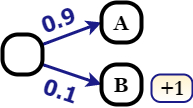
\includegraphics[width=0.15\textwidth]{Images/PrioritizedIssue.png}
%\vspace{-0.3cm}
\end{wrapfigure}

Для приоритизированного реплея, веса у переходов с $s' \HM= A$ могут отличаться от весов для переходов с $s' \HM= B$. Например, если истинное значение $V^*(s \HM A) \HM= 1, V^*(s \HM B) \HM= 1$, и мы уже выучили правильное значение $Q^*(s, a) \HM= 0.1$, то $\Loss(s, a, s'=A)$ будет равен $0.1^2$, а для $\Loss(s, a, s'=B) = 0.9^2$. Значит, $s'_1$ может появиться в переходах чаще или реже, чем с вероятностью 0.1, и это выбьет $Q(s, a)$ с её правильного значения.
\end{example}

Иными словами, приоритизированное сэмплирование приводит к \emph{смещению} (\ENGLISH{bias}). Этот эффект не так страшен поначалу обучения, когда распределение, из которого приходят состояния, всё равно скорее всего не сильно разнообразно. Более существенно нивелировать этот эффект по ходу обучения, в противном случае процесс обучения может полностью дестабилизироваться или где-нибудь застрять.

Заметим, что равномерное сэмплирование не является единственным <<корректным>> способом, но основным доступным. Мы не очень хотим <<возвращаться>> к нему постепенно с ходом обучения, но можем сделать похожую вещь: раз мы хотим подменить распределение, то можем при помощи \ENGLISH{importance sampling} сохранить тот же оптимизируемый функционал:

\begin{theorem}
При сэмплировании с приоритетами $\Prob( \T )$ использование весов $w(\T) \coloneqq \frac{1}{\Prob (\T )}$ позволит избежать эффекта смещения.
\begin{proof} Пусть $M$ --- размер буфера.
\begin{align*}
\mathbb{E}_{\T \sim \mathop{Uniform}} \Loss(\T ) &= \sum_{i=1}^M \frac{1}{M} \Loss(\T_i) = \\ 
&= \sum_{i=1}^M \Prob (\T_i) \frac{1}{M\Prob (T_i)} \Loss(\T_i) = \\
&= \mathbb{E}_{\T \sim \Prob (\T)} \frac{1}{M\Prob (\T )} \Loss(\T),
\end{align*}
что с точностью до константы $\frac{1}{M}$ и есть перевзвешивание функции потерь.
\end{proof}
\end{theorem}

\ENGLISH{Importance sampling} подразумевает, что мы берём <<интересные>> переходы, но делаем по ним меньшие шаги (вес меньше именно для <<приоритетных>> переходов). Цена за такую корректировку, конечно, в том, что полезность приоритизированного сэмплирования понижается. Раз поначалу смещение нас не так беспокоит, предлагается вводить веса постепенно: а именно, использовать веса
$$w(\T) \coloneqq \frac{1}{\Prob (\T )^{\beta(t)}}$$
где $\beta(t)$ --- гиперпараметр, зависящий от итерации алгоритма $t$. Изначально $\beta(t=0) = 0$, что делает веса равномерными (корректировки не производится), но постепенно $\beta(t)$ растёт к 1 и полностью избавляет алгоритм от эффекта смещения.

\begin{remark}
На практике веса, посчитанные по такой формуле, могут оказаться очень маленькими или большими, и их следует нормировать. Вариации, как нормировать, различаются в реализациях: можно делить веса на $\max\limits_\T w(\T)$, где максимум берётся, например, только по текущему мини-батчу, чтобы гарантировать максимальный вес 1.
\end{remark}

\subsection{Multi-step DQN}\label{subsec:multistepdqn}

DQN страдает от проблемы \emph{накапливающейся ошибки} (compound error). Условно говоря, чтобы распространить награду, полученную в некоторый момент времени, на 100 шагов в прошлое, понадобится провести 100 этапов метода простой итерации. Каждый этап мы решаем задачу регрессии в сильно неидеальных условиях, и ошибка аппроксимации накапливается.

Эта проблема, как мы увидим далее, фундаментальна для off-policy подхода. \emph{Многошаговый} (\ENGLISH{Multi-step}) --- теоретически некорректная эвристика для небольшого занижения этого эффекта. Грубо говоря, нам очень хочется распространять за одну итерацию награду сразу на несколько шагов вперёд, то есть решать многошаговые уравнения Беллмана \eqref{NstepBellman}. Мы как бы и можем уравнение оптимальности многошаговое выписать...

\begin{proposition}[$N$-шаговое уравнение оптимальности Беллмана]
\begin{equation}\label{NstepOptimBellman}
 Q^*(s_0, a_0) = \E_{\Traj_{:N} \sim \pi^* \mid s_0, a_0} \left[ \sum_{t=0}^{N-1} \gamma^{t}r_t + \gamma^N \E_{s_N} \max_{a^*_N} Q^*(s_N, a^*_N) \right]   
\end{equation}
\end{proposition}

Что мы можем сделать? Мы можем прикинуться, будто решаем многошаговые уравнения Беллмана, задав целевую переменную следующим образом:
\begin{equation}\label{Nsteptarget}
y(s_0, a_0) \coloneqq \sum_{t=0}^{N-1} \gamma^{t}r_t + \gamma^N \max_{a_N} Q^*(s_N, a_N, \theta)
\end{equation}
где $s_1, a_1 \dots a_{N-1}, s_N$ взяты из буфера. Для этого в буфере вместо одношаговых переходов $\T \coloneqq (s, a, r, s', \done)$ достаточно просто хранить другую пятёрку:
$$\T \coloneqq \left( s, \, a, \, \sum_{n=0}^{N-1} \gamma^{n}r^{(n)}, \, s^{(N)}, \, \done \right)$$
где $r^{(n)}$ --- награда, полученная через $n$ шагов после посещения рассматриваемого состояния $s$, $s^{(N)}$ --- состояние, посещённое через $N$ шагов, и, что важно, флаг $\done$ указывает на то, завершился ли эпизод в течение этого $N$-шагового роллаута\footnote{естественно, алгоритм должен рассматривать все $N$-шаговые роллауты, включая те, которые завершились за $k < N$ шагов. Для них, естественно, $r^({k'}) \HM= 0$ для $k' \HM> k$, и $Q^*(s^{(N)}, a_N) \equiv 0$ для всех $a_N$.}. Все остальные элементы алгоритма не изменяются, в частности, можно видеть, что случай $N \HM= 1$ соответствует обычному DQN.

Видно, что теперь награда, полученная за один шаг, распространяется на $N$ состояний в прошлое, и мы таким образом не только ускоряем обучение оценочной функции стартовых состояний, но и нивелируем проблему накапливающейся ошибки. 

Почему теоретически это некорректно? Беря $s_1, a_1 \dots a_{N-1}, s_N$ из буфера, мы получаем состояния из функции переходов, которая стационарна и соответствует тому мат.ожиданию, которое стоит в уравнении \eqref{NstepOptimBellman}. Но вот действия в этом мат.ожидании должны приходить из оптимальной стратегии! А в буфере $a_1, a_2 \dots a_{N-1}$ --- действия нашей стратегии произвольной давности (то есть сколь угодно неоптимальные). Вместо того, чтобы оценивать оптимальное поведение за хвост траектории (по определению $Q^*$), мы $N \HM- 1$ шагов ведём себя сколько угодно неоптимально, а затем в $s^{(N)}$ подставляем оценку оптимального поведения за хвост. Иными словами, мы недооцениваем истинное значение правой части $N$-шагового уравнения Беллмана при $N \HM> 1$. Вместо уравнения оптимальности мы решаем такое уравнение: что, если я следующие $N$ шагов веду себя как стратегия $\pi$, когда-то породившая данный роллаут, и только потом соберусь вести себя оптимально? Причём из-за нашего желания делать так в off-policy режиме $\pi$ для каждого перехода своё, то есть схеме Generalized Policy Iteration это не соответствует.

\begin{exampleBox}[righthand ratio=0.2, sidebyside, sidebyside align=center, lower separated=false]{}
Пример, когда многошаговая оценка приводит к некорректным апдейтам. На втором шаге игры в $s_1$ агент может скушать тортик или прыгнуть в лаву, и в первом эпизоде обучения агент совершил ошибку и получил огромную негативную награду. В буфер при $N \HM> 1$ запишется пример со стартовым состоянием $s_0$ и этой большой отрицательной наградой (в качестве $s^{(N)}$ будет записана лава). Пока этот пример живёт в реплей буфере, каждый раз, когда он сэмплируется в мини-батче, оценочная функция для $s_0$ обновляется этой отрицательной наградой, даже если агент уже научился больше не совершать эту ошибку и в $s_1$ наслаждается тортиками.

\tcblower
\vspace{-0.3cm}
\begin{adjustwidth}{-0.6cm}{}
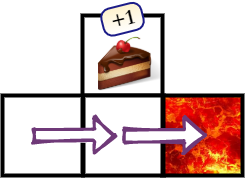
\includegraphics[width=1.15\textwidth]{Images/MultiStepBad.png} \hspace*{-1cm}
\end{adjustwidth}
\end{exampleBox}

\begin{remark}
Эмпирически большое значение $N$ действительно может полностью дестабилизировать процесс, как и подсказывает теория, поэтому рекомендуется выставлять небольшие значение 2-3, от силы 5. Большие значения могут быть работоспособны в средах, где сколько угодно неоптимальное поведение в течение $N$ шагов не приводит к существенному изменению награды по сравнению с оптимальным поведением, то есть в средах, где нет моментов с <<критическими решениями>>. 
\end{remark}